\chapter{Annotation Service Documentation}

The following two sections document the implemented functions of the ASS (section \ref{sec_B1}) and ASV (section \ref{sec_B2}) in detail. 

\section{Annotation Service Server}
\label{sec_B1}

\texttt{getDictionary()} is a utility function that fetches the dictionary associated with the current WSI/DZI from the slideDictionaries.json file\footnote{
	Compare subsection \ref{sec4_setup}
}.

It first opens slideDictionaries.json, creates a python dictionary from its content and tries to fetch the value corresponding to the WSI/DZI's name (line 2 - 4). If a value was found, it is returned (line 5 - 6), otherwise a new entry is created. The key is the WSI/DZI's file name, the value is the default dictionary from the configuration.json file, which is then returned (line 7 - 11).

\subsubsection{getDictionary()}
\begin{lstlisting}[language=Python, frame=single]
def getDictionary(file_path):
	with open(SLIDE_DICTIONARIES, 'r') as file:
		dictioary_map = json.loads(file.read())
	dictionary = dictioary_map.get(file_path)
	if dictionary:
		return dictionary
	else:
		dictioary_map[file_path] = DEFAULT_DICTIONARY
		with open(SLIDE_DICTIONARIES, 'w') as file:
			file.write(json.dumps(dictioary_map))
		return DEFAULT_DICTIONARY
\end{lstlisting}

\subsubsection{index{\textunderscore}dzi()}
If the client requests a DZI (URL ends in \emph{".dzi"}), \texttt{index{\textunderscore}dzi()} renders an ASV and passes the necessary information (slide URL, file name, MPP and dictionary) to it.

It builds the file name and slide URL (line 3 and 4) for a requested DZI. A metadata.txt will be present in the [slide name]{\textunderscore}files directory, if the DZI was created with the CS. If so, the function will try to fetch the metadata information about MPP and calculate the average size of a pixel (line 6 - 16). If the MPP metadata could not be fetched, it is set to 0 (line 17 - 18). File name, URL, MPP and dictionary are passed to the ASV, which is rendered with the given information (line 19).

\begin{lstlisting}[language=Python, frame=single]
@app.route('/wsi/<path:file_path>.dzi')
def index_dzi(file_path):
	file_name = file_path + '.dzi'
	slide_url = '/wsi/' + file_name
	# read dzi file
	try:
		with open('static/wsi/' + file_path + '_files/metadata.txt') as file:
			mpp_x = 0
			mpp_y = 0
			metadata = file.read().split('\n')
			for property in metadata:
				if openslide.PROPERTY_NAME_MPP_X in property:
					mpp_x = property.split(': ')[1]
				elif openslide.PROPERTY_NAME_MPP_Y in property:
					mpp_y = property.split(': ')[1]
			slide_mpp = (float(mpp_x) + float(mpp_y)) / 2
	except IOError:
		slide_mpp = 0
	return render_template('as_viewer.html', slide_url=slide_url, slide_mpp=slide_mpp, file_name=file_name, dictionary=getDictionary(file_name))
\end{lstlisting}


\subsubsection{index{\textunderscore}wsi()}
When the client requests a proprietary WSI (URL \emph{does not} end in ".dzi"), \texttt{index{\textunderscore}wsi()} renders an ASV and passes the necessary information (slide URL, file name, MPP and dictionary) to it. Furthermore, it wraps a DZG around the proprietary WSI and adds that to the WSGI object.

Line 1 - 8 create a map with the optional DZG parameters (compare tab. \ref{tab4_DZGparam}) and turn them into a dictionary. Line 9 reads the proprietary WSI. A DZG with the supplied parameters\footnote{Compare tab. \ref{tab4_assParams}} is created, which wraps the proprietary slide object to add Deep Zoom support (line 9 - 12). The created DZG is added to the WSGI object (line 10). Line 13 - 18 fetch associated images, the metadata (line 14), wrap the associated images with a DZG of their own and add this, together with the metadata, to the WSGI object. Line 19 - 24 fetch the MPP metadata and calculate the average MPP (or set it to 0, if not found). 
Line 25 creates a URL for the DZG object with Flasks \texttt{url{\textunderscore}for(endpoint, **values)} function. This URL is passed, together with the MPP, file path and dictionary, to an ASV which then gets rendered (line 26).

\begin{lstlisting}[language=Python, frame=single]
@app.route('/wsi/<path:file_path>')
def index_wsi(file_path):
	config_map = {
		'DEEPZOOM_TILE_SIZE': 'tile_size',
		'DEEPZOOM_OVERLAP': 'overlap',
		'DEEPZOOM_LIMIT_BOUNDS': 'limit_bounds',
	}
	opts = dict((v, app.config[k]) for k, v in config_map.items())
	slide = open_slide('static/wsi/' + file_path)
	app.slides = {
		SLIDE_NAME: DeepZoomGenerator(slide, **opts)
	}
	app.associated_images = []
	app.slide_properties = slide.properties
	for name, image in slide.associated_images.items():
		app.associated_images.append(name)
		slug = slugify(name)
		app.slides[slug] = DeepZoomGenerator(ImageSlide(image), **opts)
	try:
		mpp_x = slide.properties[openslide.PROPERTY_NAME_MPP_X]
		mpp_y = slide.properties[openslide.PROPERTY_NAME_MPP_Y]
		slide_mpp = (float(mpp_x) + float(mpp_y)) / 2
	except (KeyError, ValueError):
		slide_mpp = 0
	slide_url = url_for('dzi', slug=SLIDE_NAME)
	return render_template('as_viewer.html', slide_url=slide_url, slide_mpp=slide_mpp, file_name=file_path, dictionary=getDictionary(file_name))
\end{lstlisting}


\subsubsection{dzi(slug)}
If \texttt{index{\textunderscore}wsi()} was called before, a URL was generated for the WSI. This URL will be requested from the ASS by OpenSeadragon, which causes \texttt{slug(dzi)} to be called. \texttt{slug(dzi)} creates the DZI metadata and returns it to OpenSeadragon.

The \emph{dzi} parameter is the slide URL generated in \texttt{index{\textunderscore}wsi}.

Line 3 retrieves the format for the individual Deep Zoom tiles. Line 4 - 7 try to create a response with the requested DZI's metadata (via the DZGs \texttt{get{\textunderscore}dzi(format)} function\footnote{
	Compare subsection \ref{sec4_openslide}
}, line 5). If a response can not be created (because the requested DZG is unknown), a "404 Not Found" HTTP status code will be returned instead.\clearpage

\begin{lstlisting}[language=Python, frame=single]
@app.route('/<slug>.dzi')
def dzi(slug):
	format = app.config['DEEPZOOM_FORMAT']
	try:
		resp = make_response(app.slides[slug].get_dzi(format))
		resp.mimetype = 'application/xml'
		return resp
	except KeyError:
		# Unknown slug
		abort(404)
\end{lstlisting}


\subsubsection{tile(slug, level, col, row, format)}
If a response for OpenSeadragon was created via \texttt{slug(dzi)}, OpenSeadragon will request the individual image tiles in such a way, that, through the use of the route() decorator, \texttt{tile(slug, level, col, row, format)} will be called.

As in \texttt{slug(dzi)}, the \emph{slug} parameter is the slide URL generated in \texttt{index{\textunderscore}wsi}. The parameters \emph{level}, \emph{col} and \emph{row} describe the DZI level and address of the requested image tile. \emph{format} is the image format of the tile.

If the format is not JPEG or PNG, the ASS return a "404 Not Found" HTTP status code (line 3 - 6).

If the format is either JPEG or PNG, the requested tile is generated through the use of the DZGs \texttt{get{\textunderscore}tile(level, address)} function (line 8). If it was not possible to generate the tile, a "404 Not Found" HTTP status code will be returned.

The generated tile is then saved into a PIL image object\footnote{See \url{http://pillow.readthedocs.io/en/3.3.x/reference/Image.html}}, stored in either a JPEG or PNG image and returned as response to OpenSeadragon (line 15 - 19).

\begin{lstlisting}[language=Python, frame=single]
@app.route('/<slug>_files/<int:level>/<int:col>_<int:row>.<format>')
def tile(slug, level, col, row, format):
	format = format.lower()
	if format != 'jpeg' and format != 'png':
		# Not supported by Deep Zoom
		abort(404)
	try:
		tile = app.slides[slug].get_tile(level, (col, row))
	except KeyError:
		# Unknown slug
		abort(404)
	except ValueError:
		# Invalid level or coordinates
		abort(404)
	buf = PILBytesIO()
	tile.save(buf, format, quality=app.config['DEEPZOOM_TILE_QUALITY'])
	resp = make_response(buf.getvalue())
	resp.mimetype = 'image/%s' % format
	return resp
\end{lstlisting}


\subsubsection{saveJson()}
When the client sends JSON data to save, the \texttt{saveJson()} function is called.

The associated request is a POST request, thus the posted data must be extracted. This can be done via Flasks \emph{request object} (line 3 - 5). The file path will be transmitted as \emph{"source"}, the content to save as \emph{"json"}.

If there is content to save (line 6), it will be written into the provided file. If the file does not exist yet, it will be created (line 7 - 8).

\begin{lstlisting}[language=Python, frame=single]
@app.route('/saveJson', methods=['POST'])
def saveJson():
	dict = request.form
	source = dict.get('source', default='')
	json = dict.get('json', default='{}').encode('utf-8')
	if len(source) > 0:
		with open('static/' + source, 'w+') as file:
			file.write(json)
	return 'Ok'
\end{lstlisting}


\subsubsection{loadJson()}
When the client requests JSON data, \texttt{loadJson()} is called.

The source of the JSON data is passed in the URL as parameter (\emph{"src=[path to source]"}). The src parameter can be extracted via Flasks request object\footnote{
	Compare subsection \ref{sec4_flask}
} (line 3). If the provided source is a file, the content will be read and returned as JSON data (line 4 - 7). Otherwise an empty JSON list is returned (line 9).

\begin{lstlisting}[language=Python, frame=single]
@app.route('/loadJson')
def loadJson():
	source = 'static/wsi/' + request.args.get('src', '')
	if os.path.isfile(source):
		with open(source, 'r') as file:
			content = file.read()
			return jsonify(content)
	else:
		return jsonify('[]')
\end{lstlisting}


\subsubsection{createDictionary()}
When the client requests the creation of a new dictionary, \texttt{createDictionary()} is called. The name of the new dictionary and the associated WSI is passed as URL parameter (\emph{name= [name]} and slide=[WSI file name]). 

Once the names of dictionary and WSI were extracted (line 3- 5), the function checks if a dictionary with the provided name already exists (6 - 8). If so, \emph{"error"} is returned. Otherwise a new, empty dictionary is created (line 10 - 11). To associate the newly created dictionary to the current WSI, a key-value entry ([WSI name]:[dictionary name]) is added to the slideDictionaries.json file (13 - 17).

As response, the name and path of the newly created dictionary are returned (line 19 - 20).

\begin{lstlisting}[language=Python, frame=single]
@app.route('/createDictionary')
def createDictionary():
	name = request.args.get('name', '')
	slide = request.args.get('slide')
	path = 'static/dictionaries/' + name
	if os.path.isfile(path):
		# dictionary already exists
		return 'error'
	else:
		with open(path, 'w+') as dictionary:
			dictionary.write("[]")
	
	with open(SLIDE_DICTIONARIES, 'r') as file:
		dictioary_map = json.loads(file.read())
	dictioary_map[slide] = name
	with open(SLIDE_DICTIONARIES, 'w') as file:
		file.write(json.dumps(dictioary_map))

	respone = '{"name":"' + name + '", "path":"/' + path + '"}';
	return respone
\end{lstlisting}

\subsubsection{loadDictionary(dictionary)}

\texttt{loadDictionary(dictionary)} is called when the client requests to load a dictionary. This happens either after the creation of a new one or after switching dictionaries.

The function first builds the file path (line 3) and then checks, if a file can be found at the specified location (line 4). If not, a "404 Not Found" HTTP status code is returned (line 6). If a file could be found, its content is turned into a JSON compliant string and send to the client (line 8 - 10).

\begin{lstlisting}[language=Python, frame=single]
@app.route('/static/dictionaries/<dictionary>')
def loadDictionary(dictionary):
	dictionary = 'static/dictionaries/' + dictionary
	if os.path.isfile('/' + dictionary):
		# no dictionary found
		return '404'
	else:
		# return dictionary
		with open(dictionary, 'r') as file:
		return json.dumps(file.read())
\end{lstlisting}

\subsubsection{getDictionaries()}
The \texttt{getDictionaries()} function is called, when the client requests a list of all available dictionaries.

If no dictionaries could be found, "-1" will be returned, otherwise a JSON list of all available dictionaries.

\begin{lstlisting}[language=Python, frame=single]
@app.route('/getDictionaries')
def getDictionaries():
	dir = 'static/dictionaries/'
	if os.path.isfile(dir):
		# no dictionaries found
		return '-1'
	else:
		# return dictionaries
		return json.dumps(os.listdir(dir))
\end{lstlisting}

\subsubsection{switchDictionary()}
\texttt{switchDictionary()} is used to change the association between a dictionary and a WSI in the slideDictionary.json file.

The name of the WSI (slide) and dictionary (name) are extracted via Flask's request object (line 3 - 4). The slideDictionaries.json file is read and turned into a python dictionary. [slide] and [name] are then added to the dictionary (or updated, if the pair should already be in there), which is then written back into the file (line 6 - 10).

\begin{lstlisting}[language=Python, frame=single]
@app.route('/switchDictionary')
def switchDictionary():
	name = request.args.get('name', '')
	slide = request.args.get('slide')
	
	with open(SLIDE_DICTIONARIES, 'r') as file:
		dictioary_map = json.loads(file.read())
	dictioary_map[slide] = name
	with open(SLIDE_DICTIONARIES, 'w') as file:
		file.write(json.dumps(dictioary_map))
	
	return '200'
\end{lstlisting}

\subsubsection{runSegmentation()}
The \texttt{runSegmentation()} function is called, when the client tags a POI. It imports the python script provided in the configuration file\footnote{
	Compare tab. \ref{tab4_assConfig} in subsection \ref{sec4_setup}.
} as module and calls the module's \texttt{run(x,y)} function.

The function uses Flasks \emph{request object} to acquire the provided x and y coordinates from the provided URL (line 3 \& 4). It then opens the configuration file and extracts the name of the segmentation script (line 5 - 7). If no name was provided for the script (string is empty) the server will print an error message and return with a "404 Not Found" HTTP status code (line 8 - 10).

If a script name was provided and successfully extracted, it is imported as python module (line 12). If the import was successful, the script's run method is called and the returned contour will be passed back to the server as JSON data (line 13 - 14).

If the script could not be imported, a error message will be printed by the server and a "404 Not Found" HTTP status code is returned (line 15 - 17).

\begin{lstlisting}[language=Python, frame=single]
@app.route("/runSegmentation")
def runSegmentation():
	x = request.args.get('x', '0')
	y = request.args.get('y', '0')
	with open("static/configuration.json", 'r') as file:
		config = json.loads(file.read())
		module_name = config.get("segmentationScript")
	if(len(module_name) == 0):
		print("ERROR: no segmentation script provided in configuration file (configuration.json)!")
		return "404"
	try:
		module = __import__("static.segmentation.%s" % (module_name), fromlist=["segmentation"])
		contour = module.run(x,y)
		return json.dumps(contour)
	except ImportError:
		print("ERROR: provided segmentation script (" + module_name) not found!")
		return "404"
\end{lstlisting}


\section{Annotation Service Viewer}
\label{sec_B2}
Since the ASV has \textgreater 2,000 lines of code, there will be no documentation of every single line of code. Instead, a brief description of every function is provided. The implementation of the ASV can be found on the disc at the end of this thesis (see appendix \ref{secA_cd}).


\subsection{Initialization functions}

\subsubsection{function init(file{\textunderscore}name, url, mpp)}
\emph{Parameters:\\
	file{\textunderscore}name: name of the requested WSI\\
	url: URL to the DZI's metadata file\\
	mpp: microns per pixel of the requested WSI\\ \\
}
The \texttt{init(file{\textunderscore}name, url, mpp)} is called by the \emph{as{\textunderscore}viewer.html} to start the initialization of the ASV JavaScript. The parameters are served by the ASS. \emph{file{\textunderscore}name} describes the name of the WSI, \emph{url} contains the URL to the DZI metadata file and \emph{mpp} equals the microns per pixel of the requested WSI (if that information could be retrieved from the metadata, 0 otherwise).

The function requests the content of the configuration file (via \texttt{loadConfiguration()}) from the ASS and creates the OSDV (via \texttt{initAnnotationService()}, see fig. \ref{figB_init}).

\begin{figure}[H]
	\begin{center}
		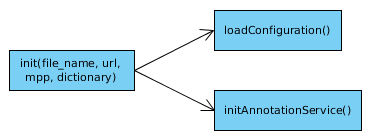
\includegraphics[scale=0.5]{img/ch_init.png}
		\caption{Call hierarchy of \texttt{init(file{\textunderscore}name, url, mpp)}}
		\label{figB_init}
	\end{center}
\end{figure}


\subsubsection{function initAnnotationService()}
\texttt{initAnnotationService()} selects the navigation tool (via \texttt{selectTool()}), creates the OSDV and its scalebar. It then opens the tile source at the URL specified in the \texttt{init(file{\textunderscore}path, url, mpp)} function. Additionally, event handlers to are set up to react to:
\begin{itemize}
	\item mouse interaction
	\item opening of a WSI
	\item zooming
\end{itemize}
Furthermore, the toolbar is initialized.

Once a tile source was opened, the AO is initialized (via \texttt{initAnnotationOverlay()}) and the saved annotations are requested (via \texttt{loadJson()}, see fig. \ref{figB_initAS}).

\begin{figure}[H]
	\begin{center}
		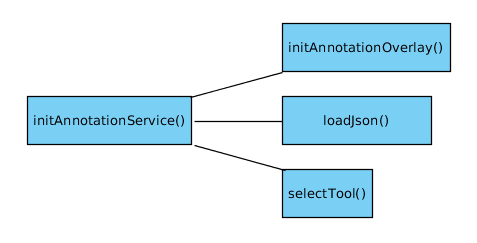
\includegraphics[scale=0.5]{img/ch_initAS.png}
		\caption{Call hierarchy of \texttt{initAnnotationService()}}
		\label{figB_initAS}
	\end{center}
\end{figure}


\subsubsection{function initAnnotationOverlay()}
\texttt{initAnnotationOverlay()} creates the ASV's AO. The AO is transformed to the size of the OSDV via the \texttt{transform()} function.


\subsection{Data management functions}

\subsubsection{function saveConfig()}
\texttt{saveConfig()} calls \texttt{saveJson(json, filePath)} to save the current configuration to the configuration file (see fig. \ref{figB_saveConfig}).

\begin{figure}[H]
	\begin{center}
		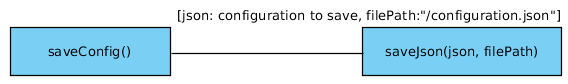
\includegraphics[scale=0.5]{img/ch_saveConfig.png}
		\caption{Call hierarchy of \texttt{saveConfig()}}
		\label{figB_saveConfig}
	\end{center}
\end{figure}


\subsubsection{function loadConfiguration()}
\texttt{loadConfiguration()} requests and parses the content of the configuration file from the ASS. Furthermore, it requests the list of available dictionaries (via \texttt{getDictionaryList()}) and loads the content of the dictionary specified in the configuration (via \texttt{loadDictionary(path)}, see fig. \ref{figB_loadConfig}).

\begin{figure}[H]
	\begin{center}
		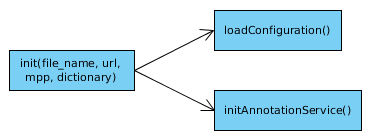
\includegraphics[scale=0.5]{img/ch_init.png}
		\caption{Call hierarchy of \texttt{loadConfiguration()}}
		\label{figB_loadConfig}
	\end{center}
\end{figure}


\subsubsection{function getDictionaryList()}
\texttt{getDictionaryList()} requests a list of all dictionaries from the ASS. The received list is then added as a clickable list to the toolbar.


\subsubsection{function saveDictionary()}
\texttt{saveDictionary()} calls \texttt{saveJson(json, filePath)} to save the current dictionary to the currently active dictionary's file (see fig. \ref{figB_saveDict}).

\begin{figure}[H]
	\begin{center}
		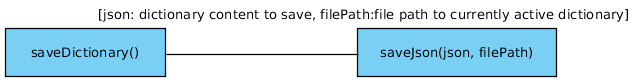
\includegraphics[scale=0.5]{img/ch_saveDict.png}
		\caption{Call hierarchy of \texttt{saveDictionary()}}
		\label{figB_saveDict}
	\end{center}
\end{figure}


\subsubsection{function loadDictionary(path)}
\emph{Parameters:\\
	path: file path of the requested dictionary\\ \\
}
\texttt{loadDictionary(path)} requests the content of the dictionary file at \emph{path} from the ASS. The response is either a list of entries, which are then added to the list of available labels in the toolbar (via \texttt{appendLabelsToList()}), or a -1, if no dictionary was found. In this case, the ASV forces the user to create a new, empty dictionary (via \texttt{createNewDictionary(isCancelable)}, see fig. \ref{figB_loadDict}).

\begin{figure}[H]
	\begin{center}
		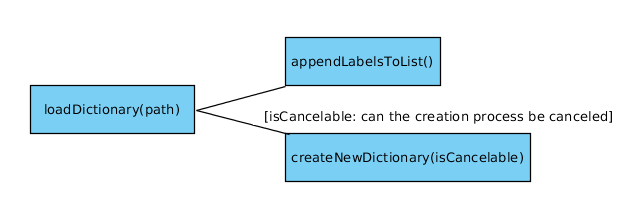
\includegraphics[scale=0.5]{img/ch_loadDict.png}
		\caption{Call hierarchy of \texttt{loadDictionary(path)}}
		\label{figB_loadDict}
	\end{center}
\end{figure}


\subsubsection{function saveJson(json, filePath)}
\emph{Parameters:\\
	json: json data to save\\
	filePath: path to the file where json should be saved\\ \\
}
\texttt{saveJson(json, filePath)} sends a POST request to the ASS with the provided json data to save and the path of the file to save the data to.


\subsubsection{function saveRegions()}
\texttt{saveRegions()} calls \texttt{saveJson(json, filePath)} to save the ASV's annotations to a file (see fig. \ref{figB_saveRegs}).

\begin{figure}[H]
	\begin{center}
		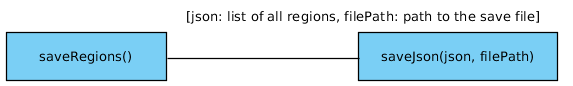
\includegraphics[scale=0.5]{img/ch_saveRegs.png}
		\caption{Call hierarchy of \texttt{saveRegions()}}
		\label{figB_saveRegs}
	\end{center}
\end{figure}


\subsubsection{function loadJson()}
\texttt{loadJson()} requests the saved annotations for the provided WSI. If an annotation file could be loaded by the ASS, a list of region data is returned. Each entry of the region data list is then turned into an actual region and added to the region list (via \texttt{newRegion(arg, imageNumber)}, see fig. \ref{figB_loadJson}).

\begin{figure}[H]
	\begin{center}
		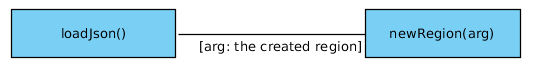
\includegraphics[scale=0.5]{img/ch_loadJson.png}
		\caption{Call hierarchy of \texttt{loadJson()}}
		\label{figB_loadJson}
	\end{center}
\end{figure}


\subsubsection{function createNewDictionary(isCancelable)}
\emph{Parameters:\\
	isCancelable: 1 if the process can be canceled without providing a valid dictionary name, 0 otherwise\\ \\
}
\texttt{createNewDictionary(isCancelable)} opens a prompt and asks the user to provide a name for the dictionary to create. If \emph{isCancelable} is true (1), the prompt can be closed and the creation process is canceled. If it is false (0), the prompt will be shown until a valid name was provided.

After creation of the new dictionary it is selected as active one (and its empty content is loaded via \texttt{loadDictionary(path)}) and the list of available dictionaries is updated (via \texttt{getDictionaryList()}, see fig. \ref{figB_createDict}).

\begin{figure}[H]
	\begin{center}
		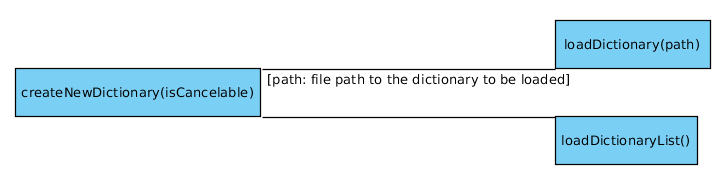
\includegraphics[scale=0.45]{img/ch_createDict.png}
		\caption{Call hierarchy of \texttt{createNewDictionary(isCancelable)}}
		\label{figB_createDict}
	\end{center}
\end{figure}


\subsection{GUI functions}

\subsubsection{function selectTool()}
\texttt{selectTool()} changes the mouse cursor to the icon of the currently selected tool.


\subsubsection{function transform()}
\texttt{transform()} resizes the AO to fit the view bounds of the OSDV.


\subsubsection{function appendLabelsToList()}
\texttt{appendLabelsToList()} first clears the currently shown list of labels. Then it iterates of the list of available labels (from the configuration) and creates a new, clickable label entry and adds it to the label list (via \texttt{appendLabelToList(label)}. Once all labels are created, the first entry is selected automatically (via \texttt{selectNextLabel()}, see fig. \ref{figB_appendLabels}).

\begin{figure}[H]
	\begin{center}
		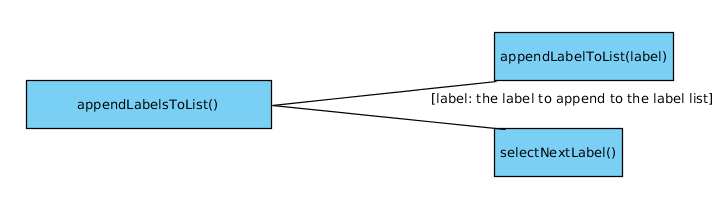
\includegraphics[scale=0.5]{img/ch_appendLabels.png}
		\caption{Call hierarchy of \texttt{appendLabelsToList()}}
		\label{figB_appendLabels}
	\end{center}
\end{figure}


\subsubsection{function appendLabelToList(label)}
\emph{Parameters:\\
	label: name of the new label
}
\texttt{appendLabelToList(label)} creates a new, clickable label for label list in the toolbar. It adds a click listener (via \texttt{singleClickOnLabel()}) to it and then selects it (via \texttt{selectLabel(el)}, see fig. \ref{figB_appendLabel}).

\begin{figure}[H]
	\begin{center}
		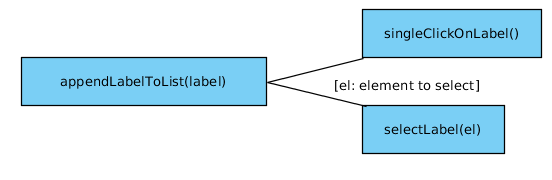
\includegraphics[scale=0.5]{img/ch_appendLabel.png}
		\caption{Call hierarchy of \texttt{appendLabelToList(label)}}
		\label{figB_appendLabel}
	\end{center}
\end{figure}


\subsubsection{function selectNextLabel()}
\texttt{selectNextLabel()} selects the next label in the toolbar list. If the currently selected label is the last one, the first entry is selected (via \texttt{selectLabel(el)}, see fig. \ref{figB_selectNextl}).

\begin{figure}[H]
	\begin{center}
		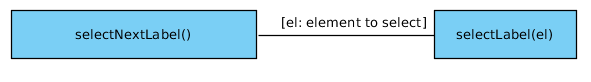
\includegraphics[scale=0.5]{img/ch_selectNext.png}
		\caption{Call hierarchy of \texttt{selectNextLabel(label)}}
		\label{figB_selectNextl}
	\end{center}
\end{figure}


\subsubsection{function selectLabel(el)}
\emph{Parameters:\\
	el: HTML element to select\\ \\
}
\texttt{selectLabel(el)} selects the provided element \emph{el} from the toolbar label list.


\subsubsection{function newLabel()}
\texttt{newLabel()} creates a new label for the toolbar's label list. The created label is also added to the dictionary and persisted there (via \texttt{saveDictionary()}). The function automatically generates a uid (via \texttt{uniqueID()}) and color (via \texttt{regionHashColor(label)}, see fig. \ref{figB_newLabel}).

\begin{figure}[H]
	\begin{center}
		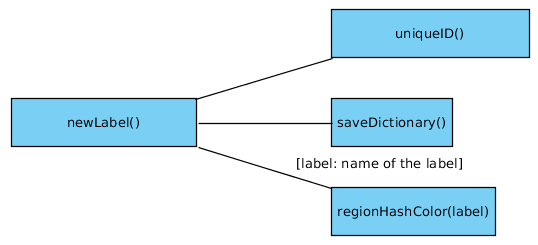
\includegraphics[scale=0.5]{img/ch_newLabel.png}
		\caption{Call hierarchy of \texttt{newLabel()}}
		\label{figB_newLabel}
	\end{center}
\end{figure}


\subsubsection{function toggleDictPicker()}
\texttt{toggleDictPicker()} toggles the visibility of the list of available dictionaries.


\subsubsection{function dictListClick(index)}
\emph{Parameters:\\
	index: index of the selected dictionary\\ \\
}
\texttt{dictListClick(index)} switches the currently active dictionary with the selected one, overwrites the currently active dictionary value in the configuration file (via \texttt{saveJson(json, filePath)}) and loads the entries from the new dictionary (via \texttt{loadDictionary(path)}, see fig. \ref{figB_selectDict}).

\begin{figure}[H]
	\begin{center}
		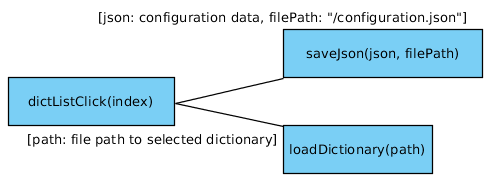
\includegraphics[scale=0.5]{img/ch_selectDict.png}
		\caption{Call hierarchy of \texttt{dictListClick(index)}}
		\label{figB_selectDict}
	\end{center}
\end{figure}


\subsubsection{function annotationStyle(label)}
\emph{Parameters:\\
	label: label whose style to modify\\ \\
}
\texttt{annotationStyle(label)} is used to manipulate the style values (stroke width and color, region color, alpha value) for the provided label.


\subsubsection{function help(show)}
\emph{Parameters:\\
	show: 1 to show help tooltip, 0 to hide it\\ \\
}
\texttt{help(show)} either shows or hides the help tooltip, depending on the provided value for show.


\subsubsection{function toggleMenu()}
\texttt{toggleMenu()} toggles visibility of the toolbar.


\subsection{Region functions}

\subsubsection{function newRegion(arg)}
\emph{Parameters:\\
	arg: argument object (either a complete region or path and coordinate information)\\ \\
}
\texttt{newRegion(arg)} creates a new region from the information provided in \emph{arg} and adds it to the region list.


\subsubsection{function selectRegion(reg)}
\emph{Parameters:\\
	reg: region to select\\ \\
}
\texttt{selectRegion(reg)} selects the provided region.


\subsubsection{function deselectRegion(reg)}
\emph{Parameters:\\
	reg: region to deselect\\ \\
}
\texttt{deselectRegion(reg)} deselects the provided region.


\subsubsection{function findContextRegion(region1)}
\emph{Parameters:\\
	region1: region to find the context to\\ \\
}
\texttt{findContextRegion(region1)} finds the context of the provided region. The label of each region that crosses, touches, surrounds or is surrounded by \emph{region1} is considered as context. Too avoid data redundancy, each label will only be added once to the context of region1 (via \texttt{isRegionAlreadyReferenced(region1, region2)}, see fig. \ref{figB_findContext}).

\begin{figure}[H]
	\begin{center}
		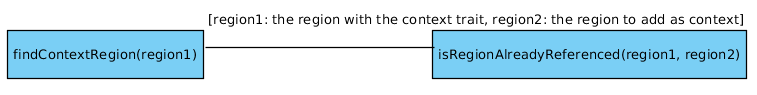
\includegraphics[scale=0.4]{img/ch_findContext.png}
		\caption{Call hierarchy of \texttt{findContextRegion()}}
		\label{figB_findContext}
	\end{center}
\end{figure}


\subsubsection{function isRegionAlreadyReferenced(region1, region2)}
\emph{Parameters:\\
	region1: region with the context to check\\
	region2: region whose label is checked for\\ \\
}
\texttt{isRegionAlreadyReferenced(region1, region2)} checks if region1's context already contains region2’s label.


\subsubsection{function removeRegion(reg)}
\emph{Parameter:\\
	reg: the region to remove\\ \\
}
\texttt{removeRegion(reg)} deletes the provided region.


\subsubsection{function findRegionByUID(uid)}
\emph{Parameter:\\
	uid: unique id of the region to find\\ \\
}
\texttt{findRegionByUID(uid)} finds a region with the provided id.


\subsubsection{function toggleRegions(uid)}
\emph{Parameters:\\
	uid: the label uid of the regions to toggle in their visibility\\ \\
}
\texttt{toggleRegions(uid)} turns all regions of the corresponding label (in-)visible. If one of the regions to be toggled is currently selected it is deselected (via \texttt{deselectRegion(reg)}, see fig. \ref{figB_toggleRegions}).

\begin{figure}[H]
	\begin{center}
		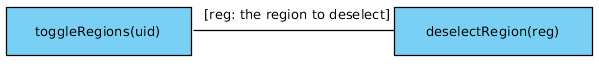
\includegraphics[scale=0.5]{img/ch_toggleRegions.png}
		\caption{Call hierarchy of \texttt{toggleRegions(uid)}}
		\label{figB_toggleRegions}
	\end{center}
\end{figure}


\subsubsection{function toggleAllRegions()}
\texttt{toggleAllRegions()} toggles the visibility of all regions.


\subsection{Interaction functions}
\subsubsection{function singleClickOnLabel(event)}
\emph{Parameters:\\
	event: the click event\\ \\
}
\texttt{singleClickOnLabel(event)} handles the click on a label in the toolbar's label list. Depending on what element inside the label is clicked, the following happens:
\begin{itemize}
	\item the visibility of all regions with the corresponding label is toggled on/off (via \texttt{toggleRegions(uid)})
	\item a window to open the annotation style (stroke width and color, alpha value, region color) is shown (via \texttt{changeRegionAnnotationStyle(uid)})
	\item the clicked label is selected (via \texttt{selectLabel(el)})
\end{itemize}

See fig. \ref{figB_singleClickLabel} for the call hierarchy of \texttt{singleClickOnLabel(event)}.

\begin{figure}[H]
	\begin{center}
		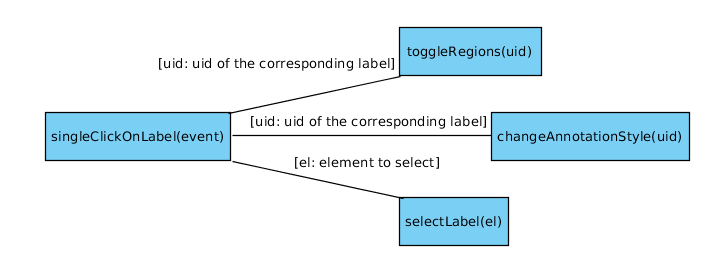
\includegraphics[scale=0.5]{img/ch_singleClickLabel.png}
		\caption{Call hierarchy of \texttt{singleClickOnLabel(event)}}
		\label{figB_singleClickLabel}
	\end{center}
\end{figure}


\subsubsection{function changeRegionAnnotationStyle(uid)}
\emph{Parameters:\\
	uid: the uid of the corresponding label\\ \\
}
\texttt{changeRegionAnnotationStyle(uid)} changes the annotation style (storke width and color, region color, region alpha value) for all regions corresponding to the label uid.


\subsubsection{function addPoi(event)}
\emph{Parameters:\\
	event: the click event\\ \\
}
\texttt{addPoi(event)} requests the server to run the segmentation script and provides it with the x and y coordinate the POI was placed at. Once the server returns with a valid answer (the image coordinates of the ROIs enclosing path), the coordinates are converted from image coordinates into AO coordinates (via \texttt{imgToPathCoordinates(point)}) and the ROI is enclosed by a path drawn along those AO coordinates. Then, a new region is created (via \texttt{newRegion(arg)}) and its checked for context (via \texttt{findContextRegion(region1)}).

If the ASS returns a "404 Not Found", an alert is shown and the currently selected POI tool is reset to the navigation tool (via \texttt{clearToolSelection()}).

Fig. \ref{fig_Bpoi} shows the call hierarchy of \texttt{addPoi(event)}.

\begin{figure}[H]
	\begin{center}
		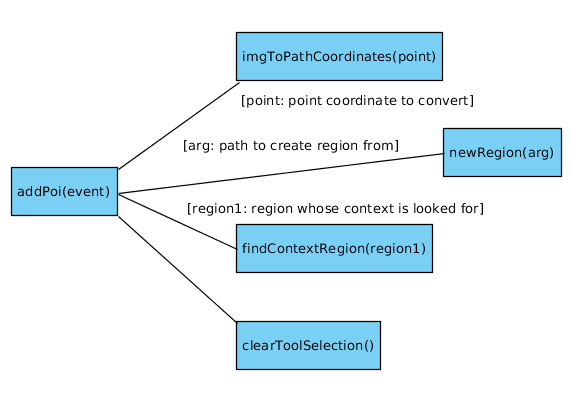
\includegraphics[scale=0.5]{img/ch_addPoi.png}
		\caption{Call hierarchy of \texttt{addPoi(event)}}
		\label{fig_Bpoi}
	\end{center}
\end{figure}


\subsection{Internal functions}

\subsubsection{UniqueID()}
\texttt{UniqueID()} creates a unique id and returns it.


\subsubsection{function regionHashColor(name)}
\emph{Parameters:\\
	name: name of a label\\ \\
}
\texttt{regionHashColor(name)} generates a color (rgba, with a = default alpha from configuration) from the hash value of the provided name.

\subsubsection{function convertPathToImgCoordinates(point)}
\emph{Parameters:\\
	point: point coordinate to convert\\ \\
}
\texttt{convertPathToImgCoordinates(point)} converts a point coordinate from the AO to a point coordinate in the OSDV's image.


\subsubsection{function convertImgToPathCoordinates(point)}
\emph{Parameters:\\
	point: point coordinate to convert\\ \\
}
\texttt{convertImgToPathCoordinates(point)} converts a point coordinate from the OSDV's image to a point coordinate in the AO.

\subsubsection{function mouseDown(x,y)}
\emph{Parameters:\\
	x: x coordinate of when left mouse button was pushed down\\
	y: y coordinate of when left mouse button was pushed down\\ \\
}
\texttt{mouseDown(x,y)} listens to mouse click events. It is called, once the mouse button is pushed down. The function handles every interaction the following interactions:
\begin{itemize}
	\item create region in free hand and polygon drawing mode (via \texttt{newRegion(arg)})
	\item add a new segment to a path in polygon drawing mode
	\item close a region's path in polygon mode, once a segment is clicked the second time (via \texttt{finishDrawingPolygon(closed)})
	\item select a clicked region (via \texttt{selectRegion(reg)})
\end{itemize}

See fig. \ref{figB_mouseDown} for the call hierarchy of \texttt{mouseDown(x,y)}.

\begin{figure}[H]
	\begin{center}
		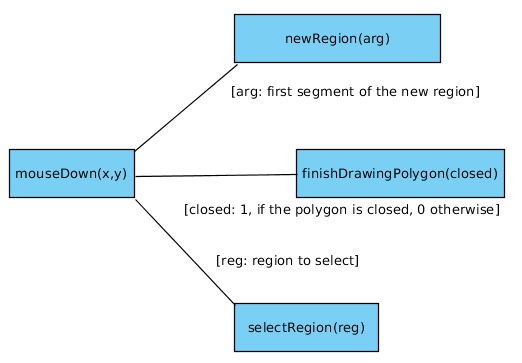
\includegraphics[scale=0.5]{img/ch_mouseDown.png}
		\caption{Call hierarchy of \texttt{mouseDown(x,y)}}
		\label{figB_mouseDown}
	\end{center}
\end{figure}


\subsubsection{function mouseDrag(x,y,dx,dy)}
\emph{Parameters:\\
	x: x coordinate with current mouse position\\
	y: y coordinate with current mouse position\\
	dx: delta of current and former mouse position in x \\
	dy: delta of current and former mouse position in y\\ \\
}
\texttt{mouseDrag(x,y,dx,dy)} handles all mouse interaction that happens with a pushed down left mouse button:
\begin{itemize}
	\item add new segment to path in free hand drawing mode (including conversion image coordinate $\rightarrow$ AO coordinate and AO coordinate $\rightarrow$ image coordinate\footnote{
		See subsection \ref{sec4_asvFrameworks} - Paper.js.
	}, see fig. \ref{figB_mouseDrag})
	\item move region
	\item move segment in region
\end{itemize}

\begin{figure}[H]
	\begin{center}
		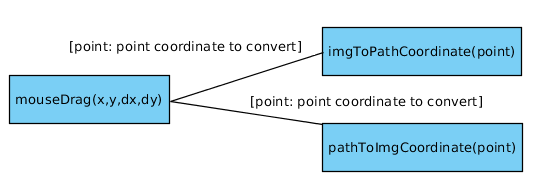
\includegraphics[scale=0.5]{img/ch_mouseDrag.png}
		\caption{Call hierarchy of \texttt{mouseDrag(x,y,dx,dy)}}
		\label{figB_mouseDrag}
	\end{center}
\end{figure}


\subsubsection{function mouseUp()}
When in free hand drawing mode, the \texttt{mouseUp()} function closes a region's path, once the left mouse button is released (including conversion as in the first item of \texttt{mouseDrag(x,y,dx,dy})).

When in distance measurement mode, the distance tooltip is removed upon release of the left mouse button.


\subsubsection{function finishDrawingPolygon(closed)}
\emph{Parameters:\\
	closed: 1 if path should be closed, 0 otherwise\\ \\
}
\texttt{finishDrawingPolygon(closed)} finishes the drawing process of a region's path in polygon drawing mode. If closed is true (1), the first and last segment will be connected.


\subsubsection{function getDistance()}
\texttt{getDistance()} calculates the euclidian distance $d$ between pixels $p_a$ and $p_b$ (see eq. \ref{eq:distance}\cite{Strang03}) of a special path called \emph{ruler} that is exclusively used for the distance measurement tool.
\begin{equation}\label{eq:distance}
	d = \sqrt{
	 	(p_b.x - p_a.x)^2 + (p_b.y - p_a.y)^2
	}
\end{equation}


\subsubsection{function clearToolSelection()}
\texttt{clearToolSelection()} resets the mouse cursor to the default icon.


\subsection{Key listener}

\subsubsection{\$(document).keydown(function(e))}
\emph{Parameters:\\
	e: key event\\ \\
}
\texttt{\$(document).keydown(function(e))} is used to handle the tool selection via hotkeys. A tool is selected depending on the keys pressed (via \texttt{selectToolOnKeyPress(id)}), see fig. \ref{figB_keyDown}).

\begin{figure}[H]
	\begin{center}
		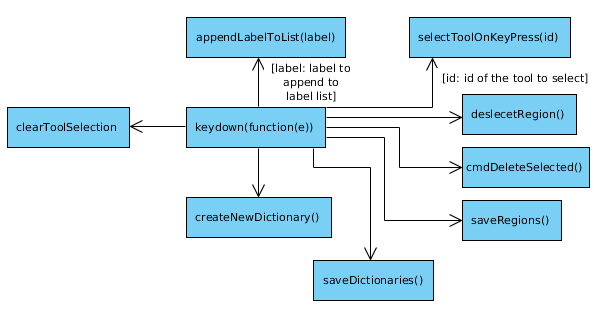
\includegraphics[scale=0.5]{img/ch_keyDown.png}
		\caption{Call hierarchy of \texttt{keydown(function(e))}}
		\label{figB_keyDown}
	\end{center}
\end{figure}
	

\subsubsection{\$(document).keyup(function(e))}
\texttt{\$(document).keyup(function(e))} resets the selected tool to the navigation tool upon release of a hotkey (via \texttt{clearToolSelection()}, see fig. \ref{figB_keyup}).

\begin{figure}[H]
	\begin{center}
		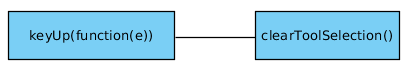
\includegraphics[scale=0.5]{img/ch_keyup.png}
		\caption{Call hierarchy of \texttt{keyup(function(e))}}
		\label{figB_keyup}
	\end{center}
\end{figure}


\subsubsection{function selectToolOnKeyPress(id)}
\emph{Parameters:\\
	id: id of the tool to select\\ \\
}
\texttt{selectToolOnKeyPress(id)} selects the tool corresponding to the provided id and changes the mouse cursor accordingly (via \texttt{selectTool()}, see fig. \ref{eq:distance}).

\begin{figure}[H]
	\begin{center}
		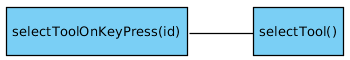
\includegraphics[scale=0.5]{img/ch_selectToolOnKeyPress.png}
		\caption{Call hierarchy of \texttt{selectToolOnKeyPress(id}}
		\label{figB_selectToolOnKeyPress}
	\end{center}
\end{figure}

